\section{Introduction}
\label{s:Literature-Introduction}
Documentation is a crucial aspect of the development of software. It is so
important that every developer building a GraphQL API should be aware of it an
keeping their Schemas documented to enable and facilitate consumers to
understand how to use the API \citep{derksDocumentingGraphQLAPIs2021}. A very a
good way to document such APIs is not to be locked in with any vendor-specific
that generates documentation on the fly given a specific schema but building
static documentation that automatically updates on the fly when a change is made
to it (ibid). The following literature review will point the differences between
different APIs, analyse and critically evaluate the options developers have to
reach the same goal and why the software implementation of the tool used in the
project gives the producers better results, freedom and save them money. Security
implications are also another important aspect of the lifecycle and this paper
will dive into analysis and confrontation to understand this.


\section{GraphQL Security}
\label{s:GraphQLSecurity}

\section{GraphQL vs REST}
\label{s:GraphQLvsRest}

Before diving in, context needs to be added on why the projects build solutions
for GraphQL instead of REST. REST has become the common choice to build and
design APIs in the past years \citep{britoRESTVsGraphQL2020}, but as the
developers needed more flexibility on evolution, a sharp decouple between the
backend and frontend and a gateway to access all the data they needed through a
single point of access. GraphQL came to the rescue of such developers wanting a
better way to build API. While REST usually have multiple endpoints to fetch
different type of data, GraphQL unifies everything through a single query to the
server with a simple JSON return with the data requested by the consumer. One of
the biggest problems of REST is overfetching. Designing an API that returns
exactly what the consumer wants in REST requests is impossible
\citep{seabraRESTGraphQLPerformance2019}. GraphQL solved the overfetching
problem as the user can write a specific query with the data needed. As
previously mentioned, GraphQL - differently from REST - is decoupled from the
backend. That means the front end can change its UI without changing the back
end for adjustments. Not only for the same reason, but the backend also has
instrumental analytics on the data requested by the consumer since everything
will be requested through a specific query. That leads to supporting graceful
deprecation of specific fields that are not mainly used. That is alluring, but
how does a consumer know which query to write to gather his data? This is when
Introspection comes in handy, but it has some critical drawbacks and security
implications that makes it unusable in production. Contrary to all the
advantages previously explained, the team at
\citet{stablekernelAdvantagesDisadvantagesGraphQL2021} also emphasised many
disadvantages. One of that is that every query always returns a state of 200
even if the query was not successful. It is very accurate and changes the way of
monitoring and measuring errors from how everyone is used with REST. GraphQL is
also very bad at handling caching which is also very complex to implement and
manage, but one thing that has not been mentioned from
\citet{stablekernelAdvantagesDisadvantagesGraphQL2021} is that it is also fairly
simple to wrap the whole API in a Content Delivery Network (CDN) that would be
the first point of contact between the server and the consumer. There are many
very viable techniques that would make this solution not only a patch to what
GraphQL does badly, but also to generally improve the API. A CDN could fully
cache any document and not only small pieces of it, making it very fast, secure,
scalable and on edge, which is always a great addition to services such as an
API.

\subsection{Introspection}
\label{s:Literature-Introspection}

Introspection is a GraphQL feature that, if enabled, grant access to a query
that returns any possible query and updates as the schema evolves overtime. A
bad actor could easily access sensitive information, types, and operations
supported with such a tool.

\begin{figure}[ht]
	\centering
	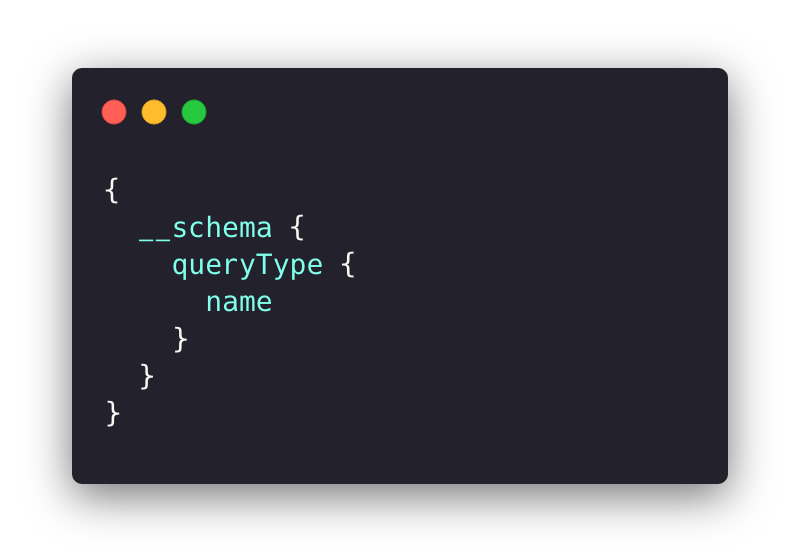
\includegraphics[width=0.5\textwidth]{figures/code/introspection.png}
	\caption{Introspection Query}
	\label{f:Introspection-Query}
\end{figure}

Introspection enables users to query a GraphQL API and discover its schema
structure, giving bad actors a chance to find potentially malicious operations
\citep{khalilWhyYouShould2021} quickly and disrupt the availability of the API.
However, it is also a requirement for tools such as \textit{GraphiQL} and
\textit{Playground}. This is a severe dilemma for producers who want to keep
their APIs as secure as possible, away from indiscreet eyes, and closed to
potential threats but still have documentation tooling. If the attackers have
access to the whole schema through introspection, it will be effortless to find
and exploit API calls meant for internal use and debugging purposes
\citep{rizwanGraphQLCommonVulnerabilities2021}. Through the same technique, the
attackers could also get access to mutations and API calls intended to add, edit
or delete specific data on the database, making it a real threat. Many other
security issues are linked to the activation of the introspection and
misconfiguration; some are information disclosure, insecure direct object
references, and inexistent Access Control List (ACL) \citep{
yeswehackHowExploitGraphQL2021}.

\subsection{N+1 Problem}
\label{s:N1-Problem}
By design, GraphQL has a fetching inefficiency known as \textit{N+1 Problem}
where the number of queries executed against the database (or other upstream
services) can be as large as the number of nodes in the resulting graph \citep{
graphqlbypopSuppressingProblemGraphQL2020}.
\begin{figure}[H]
  \centering
  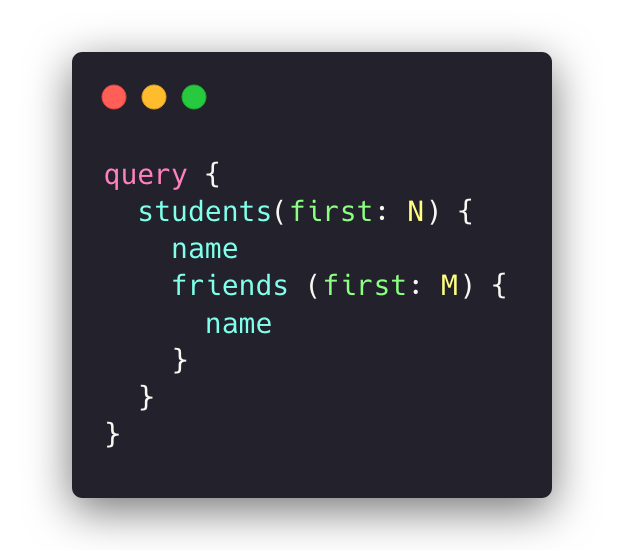
\includegraphics[width=0.5\textwidth]{figures/code/n+1}
  \caption{GraphQL N+1 Problem}
  \label{f:GraphQL-N1-Problem}
\end{figure}
In the example above, the query against the schema would make a single call to
the database to retrieve the first N students, and then for each of these Ns
students it would make a separate query to the same database to fetch M friends
details (N calls), hence N+1. Having introspection disabled is the right choice
looking at a security perspective, and this project will help solve the downside
of not having tools to help document the API and more.

\section{Exploring GraphQL API}
\label{s:Literature-ExploringGraphQLAPI}
There are different tools which lock-in both producers and consumers that aims
to explore a specific GraphQL API. The problem with those tools is that the
producer does not ever have the freedom and the flexibility to have a static
documentation running on a machine. Not only, most of the time the GraphQL
server needs to be communicating with the service, with introspection enabled.
Apollo Studio is a great tool to explore GraphQL APIs with just registering a
schema but it is a paid tool and does not come cheap. Also, in order to use most
of the tooling offered from Apollo, the server must be built with Apollo server
and this hugely lock the company or developer of the project to a single vendor
with huge implications in terms of flexibility and ownership of the whole
ecosystem that will be built around it. In practical terms, if a producer do
want to create a GraphQL API in Elixir using Absinthe \citep{
hexdocsOverviewAbsintheV12022}, it will be impossible for the developer to
utilise any of the Apollo tooling.

\section{Framework Agnostic}
\label{s:Framework Agnostic}
As previously mentioned, the end goal is to build a framework agnostic tool,
meaning that using a single GraphQL schema as a source of truth, the tool will
generate a well structured set of markdown files to document the API and utilise
those files in any way the developer wants. This would boost productivity and
flexibility as the developers can utilise the deep knowledge they already have
on a framework of their choice, with the language of their choice \citep{
stefanReasonsWhyWent2018}.

\section{GraphQL Schema}
\label{s:Literature-GraphQLSchema}
A GraphQL schema is a set of structured rules that express requirements for an
application. It might be easy with a simple UI but it can easily become
difficult as the interface of the application grows and evolves. It is to keep
in mind that most of the benefits that GraphQL brings to the table are
attributed to the schema itself as it enabled most of the features that GraphQL
provides such as code generation, parsing, validation and type checking. For
this exact reason, many developers couple GraphQL with a strong typed language
such as TypeScript to have an ecosystem of tools at their disposal that can help
them catch errors at runtime through the IDE or editor itself, rather than at
compile time. The GraphQL schema is also a graph because not only is a
representation of data graph but also a definition of relationships between
entities \citep{karthicDesigningGraphQLSchemas2020}. That are few in-built
types that are covered in GraphQL which are Object, Scalar, Query and Mutation.
The Scalar types that GraphQL supports are Int, Float, String, Boolean and ID.
All these specs will be covered and supported in the project as it is very
important to support all the types that are built-in GraphQL or the
documentation would fail to be procued as the schema could have types not
supported. An example of object type below.

\begin{figure}[H]
  \centering
  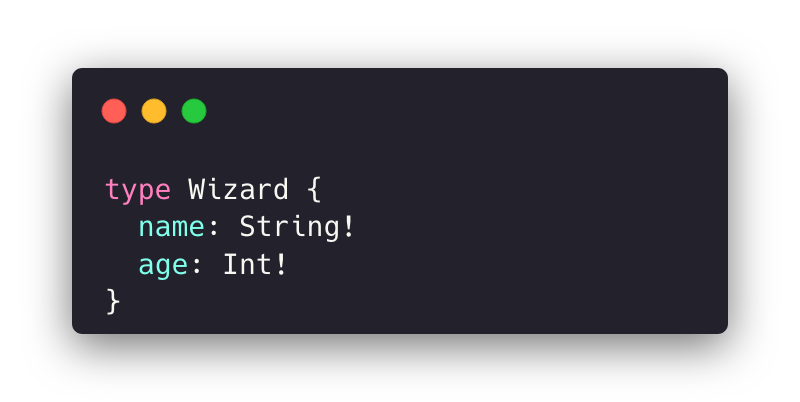
\includegraphics[width=0.5\textwidth]{figures/code/wizard}
  \caption{Object Type}
  \label{f:Wizard-Object}
\end{figure}

In this object type there are also two scalar type as field which represent
the decoration of their entities. In this case both fields are both non-nullable
fields, which means that the field cannot be null and is mandatory. Meaning that
if a consumer performs a query on a non-nullable field, he will never be able
to receive a response like the one below.

\begin{figure}[H]
  \centering
  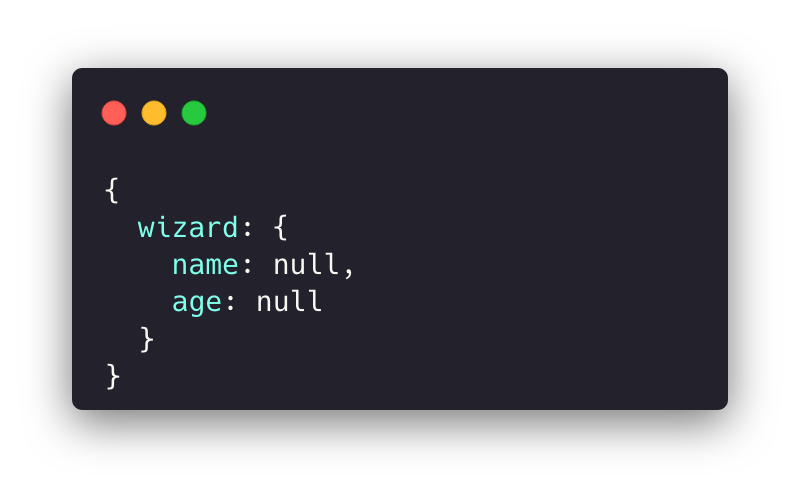
\includegraphics[width=0.5\textwidth]{figures/code/wizardresult}
  \caption{Wizard Query Result}
  \label{f:Wizard-Query-Result}
\end{figure}


\section{MD and MDX}
\label{s:MDandMDX}
As \citet{gruber38MarkdownSyntax2020} explains in his article, Markdown is
intended to be simple to read and simple to write. It is important to have a an
output text that is easy to read so that the end consumer does not have to know
anything related to coding to make things as simple as possible. In this case,
though, we also want to embed and integrate components in our markdown files,
hence the use of the MDX. It is fair to say that MDX is a superset of MD that
blends both markdown and JSX syntax to build an hybrid to power the most modern
frameworks such as React, Vue and Angular, but still leave the choice to the
developers building the project.

\section{Conclusion}
\label{s:Literature-Conclusion}
Developers are not only interested in building an API but also in continously
document it and provide a way for their consumers to have a better understanding
of the API. Even though GraphQL could have some downsides, the advantages of
using it are just far too greater to ignore. A tool to create documentation
while keeping the schema and the structure of the API secure and keeping
everything framework agnostic is something that this project will try to achieve.
After some research it is easy to say that it will be unique and could be
interesting to see how it could expand after making it open-source.
